\newpage
\section{Torque Sensor}
The purpose of the Torque Sensor is to measure the mechanical power which is given to the sensor in the form of rotational energy from the Roll. The sensor must be able to measure both torque $\tau$ and angular velocity $\omega$ as the power P is given by:
\begin{equation}
	P=\omega\cdot\tau
\end{equation}
As the Torque Sensor was chosen by the customer and as it is pre-mounted on the Roll Stand, the block will not be designed but will be analysed instead.

\subsection{Implementation}
The torque sensor picked by the customer is a DR-2212 Contactless Torque Sensor from Lorenz Messtechnik GmbH. The sensor is able to measure both the angular velocity and the torque applied to the input-shaft.

The torque sensor's input shaft is connected to the Roll and and the Generator's motor as seen on \vref{fig:Generator_Implementation}. The electrical outputs on the sensor are given through a 12-pin connector as seen on figure \ref{fig:Torque_pins} below.

\begin{figure}[H]
	\centering
	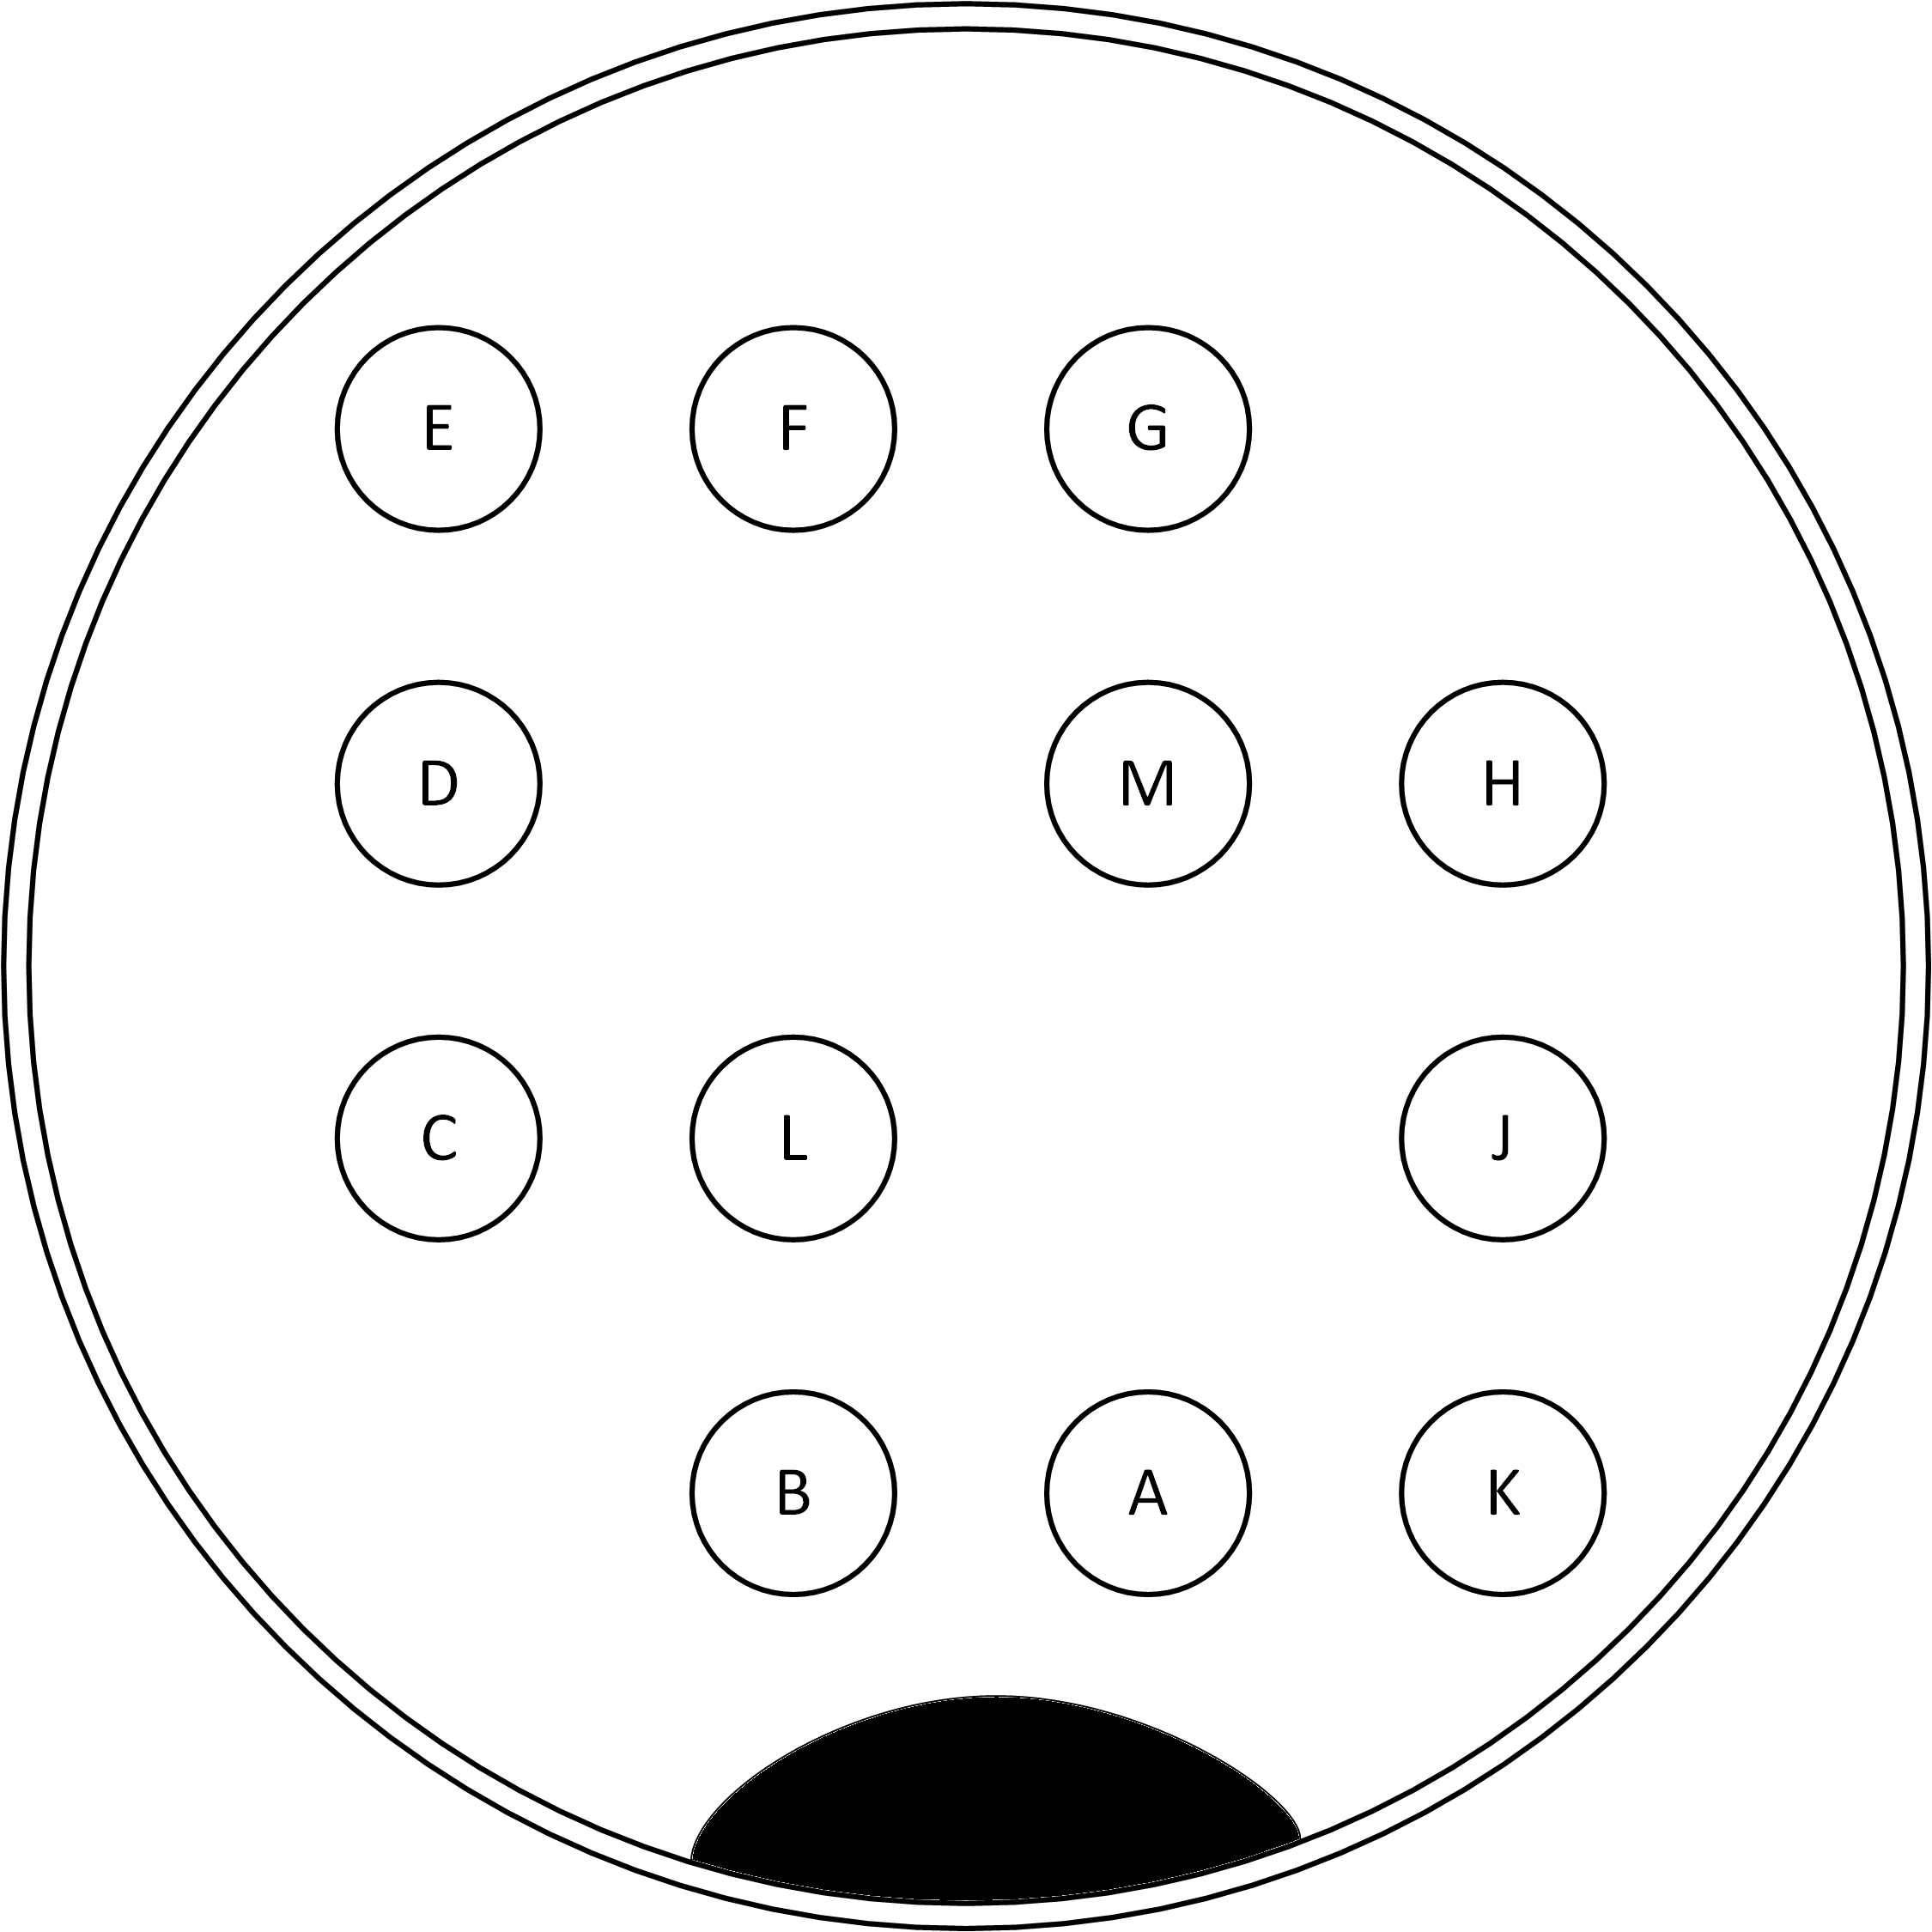
\includegraphics[width=0.4\linewidth]{Hardware/Pictures/Torque_Sensor_Pins}
	\caption{Torque Sensor pin configuration}
	\label{fig:Torque_pins}
\end{figure}

Not all 12 pins are needed to measure the torque and velocity correctly - in fact, only 5 pins are. The other end of the 12-pin cable does therefore only contain 5 connections (plus a 6th which can be used for future builds). These connections are color-coded for easy coupling with the Control-box. The connection itself is made through harwin-plugs and should be connected as specified in the table below.

\begin{table}[h]
	\centering
	\label{my-label}
	\begin{tabular}{|c|c|l|l|}
		\hline
		\textbf{Pin number} & \textbf{Pin symbol} & \multicolumn{1}{c|}{\textbf{Signal}} & \multicolumn{1}{c|}{\textbf{Color}} \\ \hline
		1                   & G                   & Velocity A                           & Grey                                \\ \hline
		2                   & C                   & Torque                               & Yellow                              \\ \hline
		3                   & F                   & Supply		                         & Brown                               \\ \hline
		4                   & E                   & Supply (GND)                         & Blue                                \\ \hline
		5                   & D                   & Torque (GND)                         & White                               \\ \hline
		6                   & B                   & Velocity B (NC)                      & Green                               \\ \hline
	\end{tabular}
	\caption{Connection between the Torque Sensor and Control-box}
\end{table}

The Torque Sensor must be supplied with atleast 12 VDC, in order to power the internal micro-processor, and can therefore be supplied directly from the Voltage Adaptor in the Control-box. The sensor could also be supplied with higher DC-voltages (up to 28 VDC), but this would require an external power supply.

\subsection{Analysis}
The sensor is specified to be able to measure torque levels ranging from 0 to \SI{5}{\newton \meter} and angular velocity from 0 to \SI{30000}{rpm}. The sensor is able to measure these parameters irregardles of the input-shaft's rotational direction. Thus the mathematical limits of the sensor range from \SI{-5}{\newton \meter} to \SI{+5}{\newton \meter} and \SI{-30000}{rpm} to \SI{+30000}{rpm}.

\textbf{Torque}\\
The Torque Sensor outputs the measured torque on Pin C (pin number 2). The output-signal is a DC-voltage which is proportional to the measured torque - as long as the input value lies withing the specified range. An input outside this range would cause the sensor to reach saturation. The output-voltage range from \SI{-5}{\volt} to \SI{+5}{\volt} and the relationship between the input and output can therefore be expressed mathematically as:
\begin{equation}
	V_{sensor} = 
	\begin{cases}
		+5V				& \quad \text{if } \tau_{sensor} > \SI{+5}{\newton \meter}\\
		\tau_{sensor}   & \quad \text{if } \SI{-5}{\newton \meter} \leq V \leq \SI{+5}{\newton \meter}\\
		-5V				& \quad \text{if } \tau_{sensor} < \SI{-5}{\newton \meter}
	\end{cases}
\end{equation}

The motor used to built the Generator is specified to handle a maximum power of \SI{200}{\watt}. This can be used to calculate the maximum torque given to the Torque Sensor's rotor, when AU2 operates at cruise speed. In the Generator's section it was found, that at AU2's cruise speed the Roll (and the sensor's input-shaft) had an angular velocity of \SI[per-mode=fraction]{109.65}{\radian \per \second}. The input-shaft's torque can then be calculated as:
\begin{equation}
	\tau_{max} = \frac{P_{max}}{\omega_{Roll}} = \frac{\SI{200}{\watt}}{\SI[per-mode=fraction]{109.65}{\radian \per \second}} = \SI{1.83}{\newton \meter}
\end{equation}
The calculated torque lies well within the specified boundaries of the Torque Sensor.

\textbf{Angular velocity}\\
The Torque Sensor outputs the measured angular velocity on Pin G (Velocity A) and Pin B (Velocity B) - however only the signal from Pin G is used for calculations. The output-signal is a square-waved signal with a DC-offset of \SI{2.5}{\volt} and a peak-peak value of \SI{5}{\volt}. The input from Pin B is connected with the Rolling Road print, but isn't connected to any kind of measuring system. The pin is only connected for potential use in future builds.

The output-signal changes level 360 times per axial revolution in the Torque Sensor. Thus the frequency of the signal is proportional to the angular velocity. The frequency of the output is given by the following equation:
\begin{equation}
	\begin{split}
		f_{sensor} = 360 \cdot \omega_{Roll}
	\end{split}
\end{equation}

\subsection{Unity test}
Text